%!  pour pdfLatex
\documentclass[a4paper]{article}
%\usepackage[hmargin={1.5cm,1.5cm},vmargin={2.4cm,2.4cm},headheight=13.1pt]{geometry}
\usepackage[a4paper,landscape,twocolumn,
            hmargin=1.8cm,vmargin=2.2cm,headheight=13.1pt]{geometry}

\usepackage[pdftex]{graphicx,color}
\usepackage[pdftex,colorlinks={true},urlcolor={blue},pdfauthor={remy Nicolai}]{hyperref}

\usepackage[T1]{fontenc}
\usepackage[utf8]{inputenc}

\usepackage{lmodern}
\usepackage[frenchb]{babel}

\usepackage{fancyhdr}
\pagestyle{fancy}

\usepackage{floatflt}
\usepackage{maths}

\usepackage{parcolumns}
\setlength{\parindent}{0pt}

\usepackage{caption}
\usepackage{subcaption}

\usepackage{makeidx}

\usepackage[french,ruled,vlined]{algorithm2e}
\SetKwComment{Comment}{\#}{}
\SetKwFor{Tq}{tant que}{}{}
\SetKwFor{Pour}{pour}{}{}
\DontPrintSemicolon
\SetAlgoLined

\usepackage{listings}
\lstset{language=Python,frame=single}
\lstset{literate=
  {á}{{\'a}}1 {é}{{\'e}}1 {í}{{\'i}}1 {ó}{{\'o}}1 {ú}{{\'u}}1
  {Á}{{\'A}}1 {É}{{\'E}}1 {Í}{{\'I}}1 {Ó}{{\'O}}1 {Ú}{{\'U}}1
  {à}{{\`a}}1 {è}{{\`e}}1 {ì}{{\`i}}1 {ò}{{\`o}}1 {ù}{{\`u}}1
  {À}{{\`A}}1 {È}{{\'E}}1 {Ì}{{\`I}}1 {Ò}{{\`O}}1 {Ù}{{\`U}}1
  {ä}{{\"a}}1 {ë}{{\"e}}1 {ï}{{\"i}}1 {ö}{{\"o}}1 {ü}{{\"u}}1
  {Ä}{{\"A}}1 {Ë}{{\"E}}1 {Ï}{{\"I}}1 {Ö}{{\"O}}1 {Ü}{{\"U}}1
  {â}{{\^a}}1 {ê}{{\^e}}1 {î}{{\^i}}1 {ô}{{\^o}}1 {û}{{\^u}}1
  {Â}{{\^A}}1 {Ê}{{\^E}}1 {Î}{{\^I}}1 {Ô}{{\^O}}1 {Û}{{\^U}}1
  {œ}{{\oe}}1 {Œ}{{\OE}}1 {æ}{{\ae}}1 {Æ}{{\AE}}1 {ß}{{\ss}}1
  {ű}{{\H{u}}}1 {Ű}{{\H{U}}}1 {ő}{{\H{o}}}1 {Ő}{{\H{O}}}1
  {ç}{{\c c}}1 {Ç}{{\c C}}1 {ø}{{\o}}1 {å}{{\r a}}1 {Å}{{\r A}}1
  {€}{{\euro}}1 {£}{{\pounds}}1 {«}{{\guillemotleft}}1
  {»}{{\guillemotright}}1 {ñ}{{\~n}}1 {Ñ}{{\~N}}1 {¿}{{?`}}1
}

%pr{\'e}sentation des compteurs de section, ...
\makeatletter
\renewcommand{\thesection}{\Roman{section}.}
\renewcommand{\thesubsection}{\arabic{subsection}.}
\renewcommand{\thesubsubsection}{\arabic{subsubsection}.}
\renewcommand{\labelenumii}{\theenumii.}
\makeatother


\newtheorem*{thm}{Théorème}
\newtheorem{thmn}{Théorème}
\newtheorem*{prop}{Proposition}
\newtheorem{propn}{Proposition}
\newtheorem*{pa}{Présentation axiomatique}
\newtheorem*{propdef}{Proposition - Définition}
\newtheorem*{lem}{Lemme}
\newtheorem{lemn}{Lemme}

\theoremstyle{definition}
\newtheorem*{defi}{Définition}
\newtheorem*{nota}{Notation}
\newtheorem*{exple}{Exemple}
\newtheorem*{exples}{Exemples}


\newenvironment{demo}{\renewcommand{\proofname}{Preuve}\begin{proof}}{\end{proof}}
%\renewcommand{\proofname}{Preuve} doit etre après le begin{document} pour fonctionner

\theoremstyle{remark}
\newtheorem*{rem}{Remarque}
\newtheorem*{rems}{Remarques}

%\usepackage{maths}
%\newcommand{\dbf}{\leftrightarrows}

%En tete et pied de page
\lhead{Informatique}
%\chead{Introduction aux systèmes informatiques}
\rhead{MPSI B Hoche}
\lfoot{\tiny{Cette création est mise à disposition selon le Contrat\\ Paternité-Partage des Conditions Initiales à l'Identique 2.0 France\\ disponible en ligne http://creativecommons.org/licenses/by-sa/2.0/fr/  
} 
\rfoot{\tiny{Rémy Nicolai \jobname \; \today } }
}
\makeindex

%En tete et pied de page
\lhead{Cours IPT}
\chead{Cours 9: Exemple base de données - Comptages routiers linéaires le 10/05/17}
\begin{document}

\section{Comptages routiers linéaires}
Le fichier (format csv) est téléchargé depuis le site\\ \href{http://opendata.hauts-de-seine.net/jeu-de-donnees/comptages-routiers-lineaires}{http://opendata.hauts-de-seine.net/jeu-de-donnees/comptages-routiers-lineaires}\\
\begin{figure}[h]
  \centering
  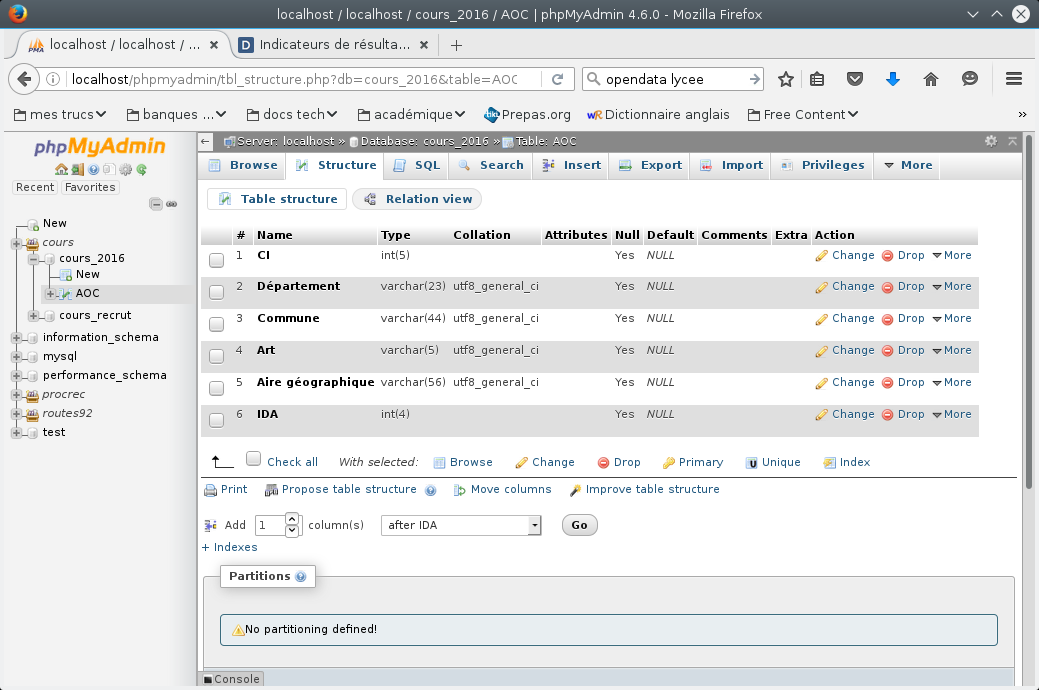
\includegraphics[width=10.5cm]{./projbdd_1.png}
  % projbdd_1.png: 593x708 pixel, 96dpi, 15.69x18.73 cm, bb=0 0 445 531
  \caption{description des champs}
  \label{fig:projbdd_1}
\end{figure}
La description des champs est donnée dans la figure \ref{fig:projbdd_1}. On commence par importer le fichier dans une base (attention le séparateur des champs est ";").
On s'intéresse aux villes figurant dans cette liste et au trafic qui en sort ou qui y entre. Elles peuvent y figurer de trois manières : comme extrémité de départ ou d'arrivée ou comme lieu de comptage. Cette table permet de former un réseau dont les noeuds sont les villes extrémités et les routes les arêtes.\\
On fera comme si tout le trafic circulant sur une route venait de la ville extrémité de départ. C'est évidemment faux mais commode pour l'exposé.
\begin{enumerate}
  \item Former une table \verb|`communes`| contenant toutes les communes quelque soit le champ dans lequel elles figurent. Que représente dans cette table la ligne dont le champ "nom" est vide ? et dans la table des comptages? Quelle décision prendre relativement à cette ligne spéciale dans la table des communes?
  \item Ajouter les champs numériques suivant dans la table des communes avec \verb|NULL| comme valeur par défaut. 
\begin{itemize}
  \item \verb|`MJO_E`| trafic moyen d'un jour ouvrable entrant cumulé pour toutes les routes.
  \item \verb|`MJO_S`| trafic moyen d'un jour ouvrable sortant cumulé pour toutes les routes.
  \item \verb|`NBR_E`| nombre de routes entrant dans une commune.
  \item \verb|`NBR_S`| nombre de routes sortant d'une commune.
\end{itemize}

  \item Calculer, à l'aide d'une requête \verb|SELECT| et de la fonction d'agrégation \verb|SUM| conditionnée par \verb|GROUP BY|, pour chaque ville, le trafic moyen cumulé entrant ou sortant. Insérer le résultat de cette requête dans une table provisoire adaptée (\verb|comm|: chaîne de 40 caractères, \verb|val|: décimal) puis mettre à jour le champ correspondant de la table des communes.

  \item Procéder de même pour les trafics moyens cumulés entrant ainsi que pour les nombres de routes entrant dans une route ou en sortant (avec la fonction d'agrégation \verb|COUNT|. 
  
  \item Recherche d'itinéraires. Tous les trajets se font dans le sens conventionnel \verb|SENS1| de la table des comptages. Un \emph{itinéraire de longueur} $l$ est une suite de $l$ routes telles que, pour $i$ entre $1$ et $l$, la ville d'arrivée de la route $i$ (notée $v_{i-1}$) soit la ville de départ de la route suivante. Un \emph{circuit} est un itinéraire dont la ville de départ est égal à la ville d'arrivée.
  \begin{enumerate}
    \item Former tous les itinéraires de longueur $2$ en précisant les routes utilisées et les moyennes des trafics moyens journaliers annuels. Filtrer tous les itinéraires de longueur $2$ qui sont des circuits. Cmprendre pourquoi certains itinéraires figurent plusieurs fois: GARCHES -> D907 -> VAUCRESSON -> D173 -> RUEIL MALMAISON par exemple.
    \item Former les itinéraires de longueur $3$ tels que $v_0 \neq v_2$. Former les circuits de longueur $3$ parmi ces itinéraires.
  \end{enumerate}
  
\end{enumerate}


\section{Requêtes}
Une remarque sur les commentaires en SQL. cela dépend du moteur. En MySQL (ou Mariadb):
\begin{itemize}
  \item \verb|#| jusqu'à la fin de la ligne
  \item Depuis \verb|/*| jusqu'à \verb|*/|. Ce type de commentaire peut s'étendre sur plusieurs lignes.
  \item Depuis \verb|-- | (double tiret espace) jusqu'à la fin de la ligne.
\end{itemize}

\begin{enumerate}
  \item Requête d'union des villes et d'insertion dans la table (déjà crée).
\begin{verbatim}
INSERT INTO `communes`
SELECT DISTINCT `SENS1_DE` FROM `comptages`
UNION
SELECT DISTINCT `SENS1_VERS` FROM `comptages`
UNION
SELECT DISTINCT `SENS2_DE` FROM `comptages`
UNION
SELECT DISTINCT `SENS2_VERS` FROM `comptages`
UNION
SELECT DISTINCT `COMMUNE` FROM `comptages`  
\end{verbatim}
\item Manipulation avec des fenêtres dans le logiciel de gestion de la base.
\item Requêtes d'agrégation. Pour calculer les trafics cumulés sortant des villes:
\begin{verbatim}
SELECT `SENS1_DE` , sum( `MJO_SENS_1` )
FROM `comptages`
GROUP BY `SENS1_DE` 
\end{verbatim}
Pour insérer dans la table provisoire ces trafics cumulés:
\begin{verbatim}
TRUNCATE `prov`; -- On commence par vider la table
INSERT INTO `prov` 
SELECT `SENS1_DE` , sum( `MJO_SENS_1` )
FROM `comptages`
GROUP BY `SENS1_DE` 
\end{verbatim}
Pour mettre à jour le champ \verb|`MJO_S`| (flux sortant) de la table des communes.
\begin{verbatim}
UPDATE `prov` 
JOIN `communes` ON `comm`=`nom`
SET `MJO_S`=`val`
\end{verbatim}

\item Pour répondre à ces questions, il faut joindre la table des routes à elle même ce qui peut se faire en utilisant des alias. 
\begin{enumerate}
  \item Requête pour trouver les itinéraires de longueur 2.
\begin{verbatim}
SELECT 
    cpt1.`SENS1_DE`, cpt1.`route`,
    cpt2.`SENS1_DE`, cpt2.`route`,
    cpt2.`SENS1_VERS`,
    (cpt1.`MJA_SENS_1`+ cpt2.`MJA_SENS_1`
 FROM comptages cpt1 
 JOIN comptages cpt2 
   ON cpt1.`SENS1_VERS`=cpt2.`SENS1_DE`
\end{verbatim}
Pour trouver les circuits de longueur 2.
\begin{verbatim}
SELECT 
  cpt1.`SENS1_DE` , cpt1.`route`,
  cpt2.`SENS1_DE` , cpt2.`route`,
  cpt2.`SENS1_VERS` 
FROM comptages cpt1 
  JOIN comptages cpt2 
    ON cpt1.`SENS1_VERS`=cpt2.`SENS1_DE` 
WHERE cpt1.`SENS1_DE`=cpt2.`SENS1_VERS`  
\end{verbatim}

  \item 
\end{enumerate}

\end{enumerate}
\end{document}